% Options for packages loaded elsewhere
\PassOptionsToPackage{unicode}{hyperref}
\PassOptionsToPackage{hyphens}{url}
%
\documentclass[
]{article}
\usepackage{amsmath,amssymb}
\usepackage{iftex}
\ifPDFTeX
  \usepackage[T1]{fontenc}
  \usepackage[utf8]{inputenc}
  \usepackage{textcomp} % provide euro and other symbols
\else % if luatex or xetex
  \usepackage{unicode-math} % this also loads fontspec
  \defaultfontfeatures{Scale=MatchLowercase}
  \defaultfontfeatures[\rmfamily]{Ligatures=TeX,Scale=1}
\fi
\usepackage{lmodern}
\ifPDFTeX\else
  % xetex/luatex font selection
\fi
% Use upquote if available, for straight quotes in verbatim environments
\IfFileExists{upquote.sty}{\usepackage{upquote}}{}
\IfFileExists{microtype.sty}{% use microtype if available
  \usepackage[]{microtype}
  \UseMicrotypeSet[protrusion]{basicmath} % disable protrusion for tt fonts
}{}
\makeatletter
\@ifundefined{KOMAClassName}{% if non-KOMA class
  \IfFileExists{parskip.sty}{%
    \usepackage{parskip}
  }{% else
    \setlength{\parindent}{0pt}
    \setlength{\parskip}{6pt plus 2pt minus 1pt}}
}{% if KOMA class
  \KOMAoptions{parskip=half}}
\makeatother
\usepackage{xcolor}
\usepackage{graphicx}
\makeatletter
\def\maxwidth{\ifdim\Gin@nat@width>\linewidth\linewidth\else\Gin@nat@width\fi}
\def\maxheight{\ifdim\Gin@nat@height>\textheight\textheight\else\Gin@nat@height\fi}
\makeatother
% Scale images if necessary, so that they will not overflow the page
% margins by default, and it is still possible to overwrite the defaults
% using explicit options in \includegraphics[width, height, ...]{}
\setkeys{Gin}{width=\maxwidth,height=\maxheight,keepaspectratio}
% Set default figure placement to htbp
\makeatletter
\def\fps@figure{htbp}
\makeatother
\setlength{\emergencystretch}{3em} % prevent overfull lines
\providecommand{\tightlist}{%
  \setlength{\itemsep}{0pt}\setlength{\parskip}{0pt}}
\setcounter{secnumdepth}{-\maxdimen} % remove section numbering
\ifLuaTeX
  \usepackage{selnolig}  % disable illegal ligatures
\fi
\usepackage{bookmark}
\IfFileExists{xurl.sty}{\usepackage{xurl}}{} % add URL line breaks if available
\urlstyle{same}
\hypersetup{
  hidelinks,
  pdfcreator={LaTeX via pandoc}}

\author{}
\date{}

\begin{document}

\section{Inizio dello sviluppo e storia
dell'algoritmo}\label{inizio-dello-sviluppo-e-storia-dellalgoritmo}

Dato che Bitcoin fallisce dal punto di vista della privacy delle
transazioni e della resistenza agli ASICs (\emph{Application Specific
Integrated Circuits}), lo sviluppatore \textbf{Nicolas van Saberhagen},
che molti pensano essere un nome di fantasia, con alcune speculazioni
che lo associerebbero al fantomatico creatore di Bitcoin,
\textbf{Satoshi Nakamoto}, nel 12 dicembre 2012 presenta un documento
con all'interno l'idea di \textbf{CryptoNote}.

Questo innovativo protocollo di consenso viene presentato come una
fattibile alternativa ai meccanismi tradizionali utilizzati dalle
criptomonete, come la \emph{Proof-Of-Work} di Bitcoin (la prova che sei
in grado di eseguire un lavoro), oltretutto in grado di garantire
elevati livelli di anonimato e un opportuna resistenza agli ASICs.
Alcune delle funzioni menzionate riguardavano transazioni di dimensione
inferiore e non facilmente associabili ad un utente, l'utilizzo delle
firme ad anello volte a migliorare la sicurezza e respingere gli
attacchi alla blockchain e l'adattamento dinamico della emissione di
moneta.

\subsection{Sviluppo dello standard CryptoNight e
adozione}\label{sviluppo-dello-standard-cryptonight-e-adozione}

Qualche mese dopo, gli sviluppatori Seigen, Max Jameson, Tuomo Nieminen,
Neocortex e Antonio M. Juarez, pubblicano un documento, facente parte
degli standard di CryptoNote, con all'interno la descrizione della
funzione di hash per la proof-of-work di CryptoNote, chiamata
\textbf{CryptoNight}.

\textbf{Bytecoin (BCN)} è stata la prima criptomoneta ad adottare il
protocollo di consenso CryptoNote, scelta giustificata dalla volontà dei
fondatori di avere una criptomoneta volta alla privacy finanziaria,
attraverso una protezione completa dell'utente che utilizza gli
strumenti finanziari messi a disposizione, dalle transazioni
all'identità personale. Come altre differenze, abbiamo l'aggiustamento
della difficoltà di minare nuova moneta ad ogni blocco, generando un
blocco ogni due minuti circa. Nonostante le buone premesse, la moneta
oggi ha un \emph{market cap} irrisorio e non è stata adottata a causa di
svariati problemi: - Inizialmente, la moneta è stata pre-minata,
fornendo l'80\% delle monete ad un gruppo di \emph{early adopters},
generando una distribuzione iniqua e sleale - Bytecoin ha avuto vari
problemi tecnici di instabilità nel corso della sua vita, con difficoltà
da parte degli utenti che partecipavano alla rete impossibilitati a
sincronizzare tutta la blockchain. - Il 20 dicembre 2017, la rete di
Bytecoin ha ricevuto un attacco DDoS massiccio, con lo scopo di rubare
le monete e distribuire la potenza tra le varie monete che adottano lo
standard CryptoNote. Gli utenti affetti erano soprattutto chi aveva un
software non aggiornato per minare nuova moneta e chi utilizzava
\emph{desktop wallets} e \emph{web wallets} si è visto rallentare o
disabilitare la sincronizzazione dei pagamenti, cosa che ha aumentato lo
sconforto dei suoi partecipanti alla rete - Non si hanno notizie
riguardo futuri sviluppi della moneta, con l'ultimo post che prometteva
lo sviluppo di una tecnologia per nascondere gli importi delle
transazioni e di creare un wallet più efficiente e sicuro, risalente al
2019.

\hfill\break
Un'altra moneta, chiamata \textbf{Monero (XMR)}, nel aprile 2014 adottò
CryptoNote, scelto per garantire la privacy e la decentralizzazione del
mining. La decisione di utilizzare questa tecnologia è stata una dei
fattori che hanno contibuito alla crescita della reputazione e al
successo di Monero come una delle monete digitali più promettenti e
utilizzate. Monero ha avuto un ruolo cruciale nello sviluppo attivo di
CryptoNight, introducendo varie modifiche al fine di adattare la
funzione alle proprie necessità. Alcune versioni utilizzate erano
specifiche per miners con risorse limitate per il mining, altre sono
state rilasciate per ottimizzare l'efficienza e l'equità del mining,
oltre a mantenere la resistenza agli ASIC. Nonostante ciò, nel 2019
Monero decise di cambiare il suo algoritmo da CryptoNote a RandomX, di
cui forniremo una descrizione data l'affinità e i prinicipi che ne
dominano lo sviluppo, oltre che risolvere una serie di problemi che si
erano sviluppati nell'algoritmo di CryptoNight.

Di seguito forniremo una panoramica sulla tecnologia CryptoNote,
presentando un approccio dettagliato e analitico per comprenderne non
solo gli aspetti funzionali e tecnici dell'algoritmo ma anche le
intrinseche necessità di migliorare lo stato corrente degli algoritmi
\emph{Proof-Of-Work}, incrementando privacy e anonimato.

\section{Aspetti tecnici di
CryptoNote}\label{aspetti-tecnici-di-cryptonote}

\subsection{Privacy e Anonimato nel Cash
Elettronico}\label{privacy-e-anonimato-nel-cash-elettronico}

Privacy e anonimato sono aspetti fondamentali del cash elettronico. I
pagamenti peer-to-peer mirano a rimanere nascosti agli occhi di terze
parti, una netta differenza rispetto alle banche tradizionali. In
generale le aziende non vogliono rivelare le loro transizioni interne e
le persone comuni desiderano mantenere riservate le proprie spese
personali.

\subsection{Proprietà di Irretracciabilità e Non
Collegabilità}\label{proprietuxe0-di-irretracciabilituxe0-e-non-collegabilituxe0}

T. Okamoto e K. Ohta hanno descritto sei criteri per un sistema di
denaro elettronico ideale, uno dei quali riguarda la privacy: la
relazione tra l'utente e i suoi acquisti deve essere irrintracciabile
{[}1\^{}{]}. Dunque, per definire il concetto di sistema di pagamento
anonimo servono due proprietà:

\begin{itemize}
\tightlist
\item
  Irretracciabilità: per ogni transizione eseguita tutti i possibili
  mittenti devono avere la stessa probabilità di essere identificati.
\item
  Non collegabilità: per due qualsiasi transizioni in uscita deve essere
  impossibile dimostrare che siano state inviate dalla stessa persona
\end{itemize}

\subsection{Limiti di Bitcoin}\label{limiti-di-bitcoin}

Bitcoin non soddisfa però il primo criterio, dato che tutte le
transazioni che avvengono sono pubbliche e possono essere ricondotte a
un\textquotesingle unica origine e ad un unico destinatario.\\
Anche se due partecipanti effettuano transazioni in modo indiretto, un
metodo di ricerca del percorso ben progettato (ad esempio, l'algoritmo
``A star'' {[}2\^{}{]}) può rivelare l'origine e il destinatario
finale.\\
Inoltre Bitcoin non sembra soddisfare neanche la seconda proprietà,
infatti, da un attenta analisi della blockchain e da alcune ricerche
{[}3\^{}{]}, {[}4\^{}{]}, {[}5\^{}{]}, si potrebbe rilevare una
connessione tra gli utenti e le loro transazioni.\\
L'incapacità di Bitcoin di soddisfare queste due proprietà ci porta a
concludere che esso non rappresenta un sistema anonimo, ma piuttosto
pseudo-anonimo. Sono state proposte diverse soluzioni {[}6\^{}{]},
{[}7\^{}{]} basate sull'idea di mescolare diverse transazioni pubbliche
e inviarle tramite un indirizzo intermediario ma questo porterebbe un
altro inconveniente, ovvero una terza parte fidata.

\subsection{Problemi del Protocollo di Consenso di
Bitcoin}\label{problemi-del-protocollo-di-consenso-di-bitcoin}

Il creatore di Bitcoin, Satoshi Nakamoto, ha descritto il protocollo di
consenso come ``un processore, un voto'', utilizzando SHA-256 per il
meccanismo di proof-of-work. Poiché gli utenti votano per determinare
l'ordine unico della cronologia delle transazioni, la correttezza e la
coerenza di questo processo sono condizioni fondamentali per l'intero
sistema. Ci sono due aspetti da sottolineare: - La rete è fuori pericolo
se il 51\% del potere di mining è sotto il controllo di utenti onesti. -
Il progresso del sistema è limitato perché se si vuole cambiare la
versione del protocollo il cambiamento avverrà solo se supportato dalla
stragrande maggioranza degli utenti {[}8\^{}{]}.

Questo permette di delineare le proprietà che una funzione di
proof-of-work deve soddisfare: non deve consentire ad un partecipante
della rete di ottenere un vantaggio significativo rispetto ad un altro,
è necesaria una sorta di equivalenza tra hardware comune e dispositivi
costisi. SHA-256 non ha queste caratteristiche: una GPU è più efficacie
di una CPU e i dispositivi ASIC sono più potenti delle GPUs
{[}9\^{}{]}.\\
Bitcoin crea quindi delle condizioni favorevoli per un ampio divario nel
potere di voto tra partecipanti, violando il principio di ``un
processore, un voto'' : i proprietari di GPU e ASIC hanno infatti molto
più potere di voto rispetto a coloro che utilizzano solo CPU.\\
\strut \\
Il sistema di script in Bitcoin è troppo complicato e pesante.
Potenzialmente consente di creare transazioni sofisticate, ma alcune
delle sue funzionalità sono disabilitate per motivi di
sicurezza{[}10\^{}{]} {[}11\^{}{]}.

\subsection{Protocolli di Firma e schemi di
CryptoNote}\label{protocolli-di-firma-e-schemi-di-cryptonote}

Seguono ora degli schemi di transazioni completamente anonime che
soddisfano le condizioni di non irretracciabilità e non collegabilità.
Una caratteristica importante è l'autonomia: il mittente non è tenuto a
collaborare con altri utenti o terze parti per le transazioni.

Lo schema di CryptoNote si basa su una primitiva crittografica chiamata
\emph{group signature}, inventata da \emph{D. Chaun} e \emph{E. van
Heyst} {[}12\^{}{]} che consente di firmare un messaggio per conto di un
gruppo.\\
Dopo aver firmato, l'utente fornisce (per verificare) non la propria
chiave pubblica, ma le chiavi di tutti gli utenti del suo gruppo. Chi
verifica vede che il vero firmatario è un membro di questo gruppo, ma
non conosce la sua esatta identità.\\
Il protocollo originale prevedeva una Terza Parte Fiduciosa (Gestore del
Gruppo), ed era l'unico che poteva risalire al reale firmatario. La
versione successiva, \emph{ring} \emph{signature}, introdotta da Rivest
{[}13\^{}{]} , prevedeva uno schema ad anello autonomo senza
responsabile del gruppo e con revoca dell'anonimato.\\
Successivamente, sono apparse diverse modifiche, quella che viene
adottata su CryptoNote per larga parte si basa sullo studio
\emph{Traceable ring signature} di E. Fujisaki and K. Suzuki
{[}14\^{}{]}.\\
Per distinguere l\textquotesingle algoritmo originale da quello
modificato nella versione su CryptoNote, quest\textquotesingle ultima
firma verrà chiamata \emph{one-time ring signature}, sottolineando la
capacità dell\textquotesingle utente di produrre una sola firma valida
con la chiave privata.\\
La proprietà di tracciabilità è stata indebolita, mantenendo però quella
di collegabilità (linkability) per fornire unicità: la chiave pubblica
potrebbe comparire in molti set di verifica esterni e la chiave privata
può essere utilizzata per generare una firma anonima unica. Nel caso di
un tentativo di doppia spesa, queste due firme saranno collegate, ma non
è necessario rivelare l'identità del firmatario.

Alla base dell'algoritmo di firma si usa EdDSA, sviluppato e
implementato da \emph{D.J. Bernstein} {[}15\^{}{]}, parametri comuni di
dominio sono: - q: numero primo; - d: elemento of Fq; - E: equazione
della curva ellittica; - G: punto base; - l: ordine primo del punto
base; - Hs: funzione hash crittografica \{0, 1\} ∗ → Fq; - Hp: funzione
hash deterministica E(Fq) → E(Fq).

Al fine di ottenere una maggiore privacy, sono necessari alcuni nuovi
termini che non dovrebbero essere confusi con le entità di Bitcoin:

\begin{itemize}
\item
  \textbf{private ec-key} è una chiave segreta standard di curva
  ellittica: un numero 𝑎 ∈ {[}1,𝑙−1{]}
\item
  \textbf{public ec-key} è una chiave pubblica standard di curva
  ellittica: un punto 𝐴=𝑎𝐺;
\item
  \textbf{one-time keypair} è una coppia di chiavi ec-private e
  ec-public;
\item
  \textbf{private user key} è una coppia \emph{(a, b)} di due diverse
  chiavi ec-private;
\item
  \textbf{tracking key} è una coppia \emph{(a, B)} di chiave ec-private
  e chiave ec-public \emph{(dove 𝐵=𝑏𝐺 e 𝑎≠𝑏)};
\item
  \textbf{public user key} è una coppia \emph{(A, B)} di due chiavi
  ec-public derivate da \emph{(a, b)};
\item
  \textbf{standard} \textbf{address} è una rappresentazione di una
  chiave utente pubblica mediante una stringa digitabile
  dall\textquotesingle utente con correzione degli errori.
\end{itemize}

La struttura generale della transazione rimane quasi identica a quella
di Bitcoin: ogni utente può scegliere diversi pagamenti (transaction
outputs), firmarli con le chiavi private corrispondenti e inviarli a
diverse destinazioni.\\
Contrariamente al modello di Bitcoin, in cui un utente possiede sia le
chiavi uniche private che pubbliche, nel modello proposto un mittente
genera una chiave one-time publica basata sull'indirizzo del
destinatario e su alcuni dati. In questo senso, una transazione in
entrata per lo stesso destinatario viene inviata a una chiave pubblica
monouso (non direttamente a un indirizzo univoco) e solo il destinatario
può recuperare la parte privata corrispondente per riscattare i suoi
fondi (utilizzando la sua chiave privata unica). Il destinatario può
spendere usando una firma ad anello, mantenendo anonima la sua proprietà
e la sua effettiva spesa.

\subsection{Funzionamento delle
transazioni}\label{funzionamento-delle-transazioni}

Gli indirizzi Bitcoin classici, una volta pubblicati, diventano
identificatori inequivocabili per ogni pagamento in entrata,
collegandoli tra loro e associandoli al destinatario.

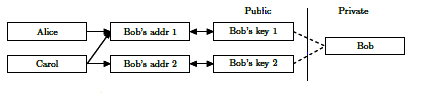
\includegraphics{media/image6.png}

Viene proposta una soluzione che consente all\textquotesingle utente di
pubblicare un singolo indirizzo e ricevere pagamenti incondizionati non
collegabili. La destinazione di ciascun output (di default) è una chiave
pubblica unica, derivata dall\textquotesingle indirizzo del destinatario
e dall\textquotesingle iniezione di dati casuali da parte del
mittente.\\

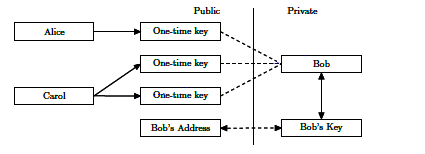
\includegraphics{media/image7.png}

Innanzitutto, il mittente esegue il protocollo di scambio Diffie-Hellman
per ottenere un segreto condiviso dai suoi dati e da una metà
dell\textquotesingle indirizzo. Successivamente calcola una chiave di
destinazione monouso, utilizzando questi segreti e la seconda metà. Per
questi due passaggi sono necessarie due chiavi ec-keys del destinatario;
quindi, un indirizzo CryptoNote standard è grande quasi il doppio di un
indirizzo Bitcoin. Il destinatario esegue anche il protocollo
Diffie-Hellman e poi recupera la chiave segreta corrispondente.

Una transazione standard procede come segue:

\begin{enumerate}
\def\labelenumi{\arabic{enumi}.}
\item
  Alice vuole inviare un pagamento a Bob, che ha pubblicato il suo
  indirizzo. Lo decomprime e ottiene la chiave utente pubblica di Bob
  \emph{(A, B)}.
\item
  Alice genera un numero casuale 𝑟 ∈ {[}1,𝑙−1{]} e calcola la chiave
  pubblica one-time 𝑃=𝐻𝑠(𝑟𝐴)𝐺+𝐵.
\item
  Alice usa 𝑃 come chiave di destinazione per l\textquotesingle output e
  inserisce anche il valore 𝑅=𝑟𝐺 (come parte del protocollo
  Diffie-Hellman) da qualche parte nella transazione. Alice può creare
  altri output con chiavi pubbliche uniche: chiavi diverse dei
  destinatari \emph{(𝐴𝑖,𝐵𝑖)} implicano 𝑃𝑖\hspace{0pt} diversi anche con
  lo stesso 𝑟.

  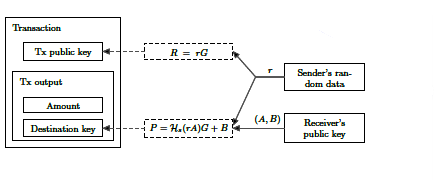
\includegraphics{media/image3.png}
\item
  Bob controlla ogni transazione in arrivo con la sua chiave privata (a,
  b), calcolando 𝑃′=𝐻𝑠(𝑎𝑅)𝐺+𝐵. Se la transazione di Alice è presente,
  allora 𝑎𝑅=𝑎𝑟𝐺=𝑟𝐴 e 𝑃′=𝑃.
\item
  Ora Bob può recuperare la chiave privata una tantum corrispondente:
  𝑥=𝐻𝑠(𝑎𝑅)+𝑏, così come 𝑃=𝑥𝐺. Può spendere questo output in qualsiasi
  momento firmando la transazione con 𝑥.

  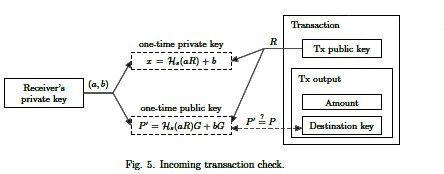
\includegraphics{media/image4.png}
\end{enumerate}

Di conseguenza, Bob riceve pagamenti in entrata associati a chiavi
pubbliche monouso che non possono essere collegate per un osservatore
esterno.

\subsubsection{Firme ad anello}\label{firme-ad-anello}

Un protocollo basato su firme ad anello monouso consente agli utenti di
ottenere un\textquotesingle anonimato incondizionato. Purtroppo, i tipi
ordinari di firme crittografiche permettono di tracciare le transazioni
ai rispettivi mittenti e destinatari. La \emph{one-time ring signature}
usa diverse tipi di firme, consiste di quattro algoritmi (\textbf{GEN,
SIG, VER, LNK}).

\begin{itemize}
\tightlist
\item
  \textbf{GEN} prende parametri pubblici e restituisce una coppia ec
  \emph{(P, x)} e una chiave pubblica I.
\item
  \textbf{SIG} riceve un messaggio m, un insieme S' di chiavi pubbliche
  \{Pi\}i≠s, le coppie \emph{(Ps, xs)} e restituisce una firma σ e un
  insieme S = S' ∪ \{Ps\}.
\item
  \textbf{VER} riceve un messaggio m, un insieme S, una firma σ e
  restituisce "true" o "false".
\item
  \textbf{LNK} riceve un insieme I = \{Ii\}, una firma σ e restituisce
  "linked" o "indep".
\end{itemize}

Lo scopo principale del protocollo è il seguente: un utente produce una
firma che può essere verificata non da una singola chiave pubblica, ma
da un insieme di chiavi. Il vero firmatario è indistinguibile dagli
altri proprietari di chiavi fino a quando non produce la seconda firma
sotto la stessa coppia di chiavi.

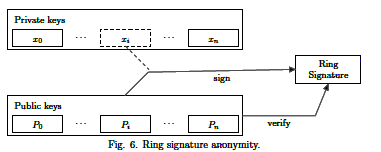
\includegraphics{media/image5.png}

\begin{itemize}
\tightlist
\item
  \textbf{GEN}: Il firmatario sceglie casualmente una chiave segreta 𝑥 ∈
  {[}1,𝑙−1{]} e calcola la chiave pubblica corrispondente 𝑃=𝑥𝐺. Inoltre,
  calcola un\textquotesingle altra chiave pubblica 𝐼=𝑥𝐻𝑝(𝑃) chiamata
  "immagine della chiave".
\item
  \textbf{SIG}: Il firmatario genera una firma ad anello one-time con
  una prova a conoscenza zero non interattiva. Seleziona un sottoinsieme
  casuale 𝑆'\hspace{0pt} di n - 1 chiavi pubbliche di altri utenti 𝑃𝑖,
  la propria coppia di chiavi (x, P) e l\textquotesingle immagine della
  chiave I. Sia 1≤𝑠≤𝑛 l\textquotesingle indice segreto del firmatario in
  S (in modo che la sua chiave sia 𝑃𝑠).\\
  Si sceglie casualmente un elemento casuale da \{qi \textbar{} i = 1
  ... n\} e \{wi \textbar{} i = 1 ... n, i ≠ s\} da (1 ... l) e effettua
  i seguenti passaggi:
  \[ L_i = \begin{cases} q_iG, & \text{se } i = s \\ q_iG+w_iP_i, & \text{se } i \neq s \end{cases} \]
\end{itemize}

\[ R_i = \begin{cases} q_iH_p(P_i), & \text{se } i = s \\ q_iH_p(P_{i})+ w_iI, & \text{se } i \neq s \end{cases} \]

Il prossimo passo è ottenere la sfida non interattiva:

\[ c = H_s(m, L_1, \ldots, L_n, R_1, \ldots, R_n) \]

Infine il firmatario calcola la risposta:

\[ c_i = \begin{cases} w_i, & \text{se } i \neq s \\ \left(c -\sum_{i=1}^{n} c_i\right) \mod l, & \text{se } i = s \end{cases} \]

\[ r_i = \begin{cases} q_i, & \text{se } i \neq s \\ q_s - c_sx \mod l ,& \text{se } i=s \end{cases} \]

La firma risultante è \[ \sigma= (I,c_1,\ldots,c_n,r_1,\ldots,r_n). \]:

\textbf{VER}: Chi sta verificando controlla la firma, ricostruendo:

\[ \begin{cases}
L_i' = r_iG + c_iP_i \\
R_i' = r_iH_p(P_i) + c_iI
\end{cases}
 \] Chi verifica controlla se
\[\sum_{i=1}^{n} ci =^? H_s(m,L_1',...,L_n',R_1',...R_n') \mod l \]

Se questa uguaglianza è vera, chi verifica esegue
l\textquotesingle algoritmo \textbf{LNK}, altrimenti respinge la firma.
- \textbf{LNK}: Chi verifica controlla se I è stata utilizzata in firme
passate (questi valori sono memorizzati nell\textquotesingle insieme I).
Un doppio utilizzo significa che sono state prodotte due firme con la
stessa chiave segreta.\\
Meccanismo del protocollo: utilizzando L-commitments, il firmatario
dimostra di conoscere un certo 𝑥 tale che almeno una 𝑃𝑖=𝑥𝐺. Per rendere
questa prova non ripetibile introduciamo l\textquotesingle immagine
della chiave come 𝐼=𝑥𝐻𝑝(𝑃). Il firmatario utilizza gli stessi
coefficienti (𝑟𝑖,𝑐𝑖) per dimostrare quasi la stessa cosa: egli conosce
un certo 𝑥 tale che almeno uno 𝐻𝑝(𝑃𝑖)=𝐼⋅𝑥\^{}−1. Se 𝑥→𝐼 è iniettiva:

\begin{verbatim}
- Nessuno può recuperare la chiave pubblica dall\'immagine della chiave
\end{verbatim}

e identificare il firmatario;

\begin{verbatim}
- Il firmatario non può fare due firme con I diverse e lo stesso x.
\end{verbatim}

Con una firma ad anello one-time, Bob può efficacemente nascondere
l'output di Alice (cioè, il suo input) tra gli altri: tutti i possibili
spenditori saranno equiprobabili, anche se Alice non ha più informazioni
di qualsiasi osservatore. Bob specifica n-1 outputs, non sapendo se
alcuni di questi sono stati spesi:\\
Un output può essere utilizzato in migliaia di firme come fattore di
ambiguità e mai come obiettivo di occultamento. Il controllo di doppia
spesa avviene nella fase LNK quando si cerca
nell\textquotesingle insieme delle immagini di chiave utilizzate.\\
Bob può scegliere il grado di ambiguità autonomamente: n = 2 significa
che avrà speso l\textquotesingle output con una probabilità del 50\%, n
= 100 dà il 1\%. La dimensione della firma risultante è lineare O(n),
quindi l\textquotesingle anonimato costa a Bob una dimensione di
transazione più grande e commissioni più alte.

Combinando entrambi i metodi (chiavi di transazione one-time e firme ad
anello one-time), Bob raggiunge un nuovo livello di privacy rispetto
allo schema originale di Bitcoin. Gli basta memorizzare una sola chiave
privata (a, b) e generare una chiave pubblica (A, B) per iniziare a
ricevere e inviare transazioni anonime. Per ogni output Bob recupera
coppie di chiavi di transazione uniche (pi, Pi) che non possono essere
collegate tra loro o alla sua chiave pubblica. Può spendere ognuna di
esse, firmando ogni input con una firma ad anello non tracciabile.

\subsection{Miglioramenti nella PoW rispetto a
Bitcoin}\label{miglioramenti-nella-pow-rispetto-a-bitcoin}

C'è stato anche un miglioramento dell'algoritmo di PoW, come obiettivo
primario vi è l'abbassamento del gap tra CPU e GPU/FPGA/ASIC.\\
Il protocollo originale di proof-of-work di Bitcoin utilizza la funzione
SHA-256.\\
Consiste principalmente di operatori logici di base e si basa
esclusivamente sulla velocità computazionale del processore, quindi è
perfettamente adatto per l\textquotesingle implementazione
multicore/conveyer. Tuttavia, i computer moderni non sono limitati solo
dal numero di operazioni al secondo, ma anche dalla dimensione della
memoria. Mentre alcuni processori possono essere notevolmente più veloci
di altri {[}9\^{}{]}, le dimensioni della memoria sono meno probabili
che varino tra le macchine.\\
L\textquotesingle idea principale è costruire un algoritmo che alloca un
ampio blocco di dati ("scratchpad") all\textquotesingle interno della
memoria e "accedere a una sequenza imprevedibile di posizioni" in esso.
Il blocco dovrebbe essere sufficientemente grande per rendere più
vantaggioso conservare i dati piuttosto che ricalcolarli ad ogni
accesso. L\textquotesingle algoritmo dovrebbe inoltre impedire il
parallelismo interno, quindi N thread simultanei dovrebbero richiedere N
volte più memoria contemporaneamente.\\
Dwork et al {[}16\^{}{]} hanno investigato e formalizzato questo
approccio, portandoli a suggerire un\textquotesingle altra variante
della funzione di pricing: "Mbound". Un altro lavoro appartiene a F.
Coelho {[}17\^{}{]}, che ha proposto la soluzione più efficace:
"Hokkaido". Con ogni probabilità, l\textquotesingle ultimo lavoro è
basato sull\textquotesingle idea di ricerche pseudo-casuali in un grande
array è l\textquotesingle algoritmo noto come "scrypt" di C. Percival
{[}18\^{}{]}. A differenza delle funzioni precedenti, si concentra sulla
derivazione delle chiavi e non sui sistemi di proof-of-work. Nonostante
ciò, scrypt funziona bene come funzione di prezzo nel problema di
conversione dell'hash parziale come SHA-256 in Bitcoin.\\
Per ora lo script è stato applicato a Litecoin {[}19\^{}{]}, ma la sua
implementazione non è veramente legata alla memoria: il rapporto ``tempo
di accesso alla memoria / tempo complessivo'' non è abbastanza grande
perché ogni istanza utilizza solo 128 KB, questo dunque permette ai
miner GPU di essere 10 volte più efficienti lasciando la possibilità di
creare dispositivi di mining efficienti e relativamente economici.\\
CryptoNote propone quindi un nuovo algoritmo memory-bound per la
proof-of-work. Si basa sull\textquotesingle accesso casuale a una
memoria lenta e sottolinea la dipendenza dalla latenza. A differenza di
scrypt, ogni nuovo blocco (lungo 64 byte) dipende da tutti i blocchi
precedenti e non solo da uno, quindi il compromesso tra dimensione della
memoria e velocità della CPU diventa esponenziale. Il nuovo algoritmo
richiede circa 2 Mb per istanza per i seguenti motivi:

\begin{itemize}
\item
  Si adatta alla cache L3 (per core) dei processori moderni, che
  diventeranno mainstream tra qualche anno;
\item
  Un megabyte di memoria interna è quasi una dimensione inaccettabile
  per il moderno pipeline ASIC;
\item
  Le GPU possono eseguire centinaia di istanze simultanee, ma sono
  limitate in altri modi: la memoria GDDR5 è più lenta della cache L3
  della CPU e notevole per la sua larghezza di banda, non per la
  velocità di accesso casuale.
\item
  Un\textquotesingle espansione significativa dello scratchpad
  richiederebbe un aumento delle iterazioni, il che implica a sua volta
  un aumento del tempo complessivo. Chiamate "pesanti" in una rete P2P
  senza fiducia possono portare a gravi vulnerabilità, perché i nodi
  sono obbligati a verificare il proof-of-work di ogni nuovo blocco. Se
  un nodo impiega una quantità considerevole di tempo per ogni
  valutazione dell\textquotesingle hash, può essere facilmente soggetto
  a attacchi DDoS da parte di una valanga di oggetti falsi con dati di
  lavoro arbitrari (valori di nonce).
\end{itemize}

\subsection{Equità nella
distibuzione}\label{equituxe0-nella-distibuzione}

Il limite superiore per l\textquotesingle ammontare complessivo delle
monete digitali CryptoNote è anche digitale:
\[\text{MSupply} = 2^{64} - 1\] unità atomiche. Questa è una restrizione
naturale basata solo su limiti di implementazione, non su intuizioni
come "N monete dovrebbero essere sufficienti per chiunque".

Per garantire la regolarità del processo di emissione, viene utilizzata
la seguente formula per le ricompense dei blocchi: \[
\text{BaseReward} = (\text{MSupply} - A) >> 18 \]

dove A è l\textquotesingle ammontare di monete generate precedentemente

CryptoNote contiene un algoritmo di targeting che cambia la difficoltà
di ogni blocco. Questo migliora il tempo di reazione del sistema quando
la potenza di calcolo della rete cresce o diminuisce intensamente,
preservando un tasso di blocco costante. Il metodo originale di Bitcoin
calcola il rapporto tra la difficoltà effettiva e quella target tra gli
ultimi 2016 blocchi e lo utilizza come moltiplicatore per la difficoltà
attuale. Ovviamente questo è inadatto per ricalcoli rapidi (a causa
dell\textquotesingle inerzia elevata) e porta a oscillazioni.
L\textquotesingle idea generale dietro l'algoritmo è sommare tutto il
lavoro completato dai nodi e dividerlo per il tempo impiegato per
completare il lavoro. La misura del lavoro sono i valori di difficoltà
corrispondenti in ogni blocco.

Gli utenti pagano gli altri per memorizzare la blockchain e dovrebbero
avere il diritto di votare per la sua dimensione. Ogni miner si
confronta con il compromesso tra bilanciare i costi e il profitto dalle
commissioni, quindi stabilisce il proprio "limite flessibile" per la
creazione dei blocchi. Inoltre, la regola fondamentale per la dimensione
massima del blocco è necessaria per evitare che la blockchain venga
inondatata da transazioni fasulle, tuttavia questo valore non dovrebbe
essere codificato duramente. Sia MN il valore mediano delle dimensioni
degli ultimi N blocchi.\\
Allora il "limite rigido" per la dimensione dei blocchi accettati è 2 ·
MN.

Un miner ha ancora la possibilità di riempire un blocco con le sue
transazioni senza commissioni fino alla dimensione massima di 2 MB.
Anche se solo la maggioranza dei miners può spostare il valore mediano,
esiste comunque la possibilità di gonfiare la blockchain e produrre un
carico aggiuntivo sui nodi. Per scoraggiare i partecipanti malevoli dal
creare blocchi grandi, introduciamo una funzione di penalità:

\[
\text{NewReward} = \text{BaseReward} \times \left( \frac{\text{DimBlocco}}{MN} - 1 \right)^2
\]

Questa regola viene applicata solo quando la DimBlocco è maggiore della
dimensione minima del blocco gratuito che dovrebbe essere vicina a \[
\max(10\, \text{kb}, M_N \cdot 110\%) \] I miners sono autorizzati a
creare blocchi di ``dimensioni usuali'' e persino a superarle con
profitto quando le commissioni complessive superano la penalità.\\
Tuttavia, è improbabile che le commissioni crescano in modo quadratico a
differenza del valore della penalità, quindi ci sarà un equilibrio.

\section{Funzione di hash
CryptoNight}\label{funzione-di-hash-cryptonight}

In questo capitolo parleremo del cuore del protocollo di consenso
CryptoNote, la funzione di hash \textbf{CryptoNight}, completa con le
sue specifiche e il suo funzionamento. L'obiettivo era il design di una
funzione che fosse facilmente eseguibile da CPU consumer-grade,
disponibili nei computer normali attraverso l'esecuzione di cifrature
AES, la moliplicazione di numeri a 64 bit e l'utilizzo di uno scratchpad
che, come da specifiche dell'algoritmo, entra nella dimensione di una
classica cache L3 di un processore dell'epoca (circa 2MB). La volontà,
più ambiziosa, era quella di rendere la funzione non facilmente
computabile dagli ASICs. Viene presentata come una funzione
\emph{memory-hard}, quindi resistente come algoritmo crittografico agli
attachi effettuati cercando di ridurre la complessità aumentando le
risorse hardware, progettata per essere inefficiente su GPU, FPGA e
ASICs rispetto alle classiche funzioni utilizzate nella
\emph{proof-of-work}, come ad esempio \emph{SHA-256}.

\subsubsection{Definizioni}\label{definizioni}

\begin{itemize}
\item
  Una \textbf{funzione di hash} è una funzione che trasforma dati di
  dimensione arbitraria in dati di dimensione fissata. L'operazione deve
  essere simile ad una funzione casuale per garantire la distribuzione
  uniforme dei risultati, indipendentemente dalla natura dei dati o
  dalle precedenti iterazioni dei dati.
\item
  \textbf{Scratchpad}: è una grande area di memoria temporanea e non
  persistente dove si possono eseguire calcoli senza alcuna conseguenza
  sullo stato a lungo termine.
\item
  \textbf{Memory-hard}: è una caratteristica delle funzioni di hash per
  il quale sono difficili da invertire, cioè trovare il dato originale a
  partire dal suo output, anche se si hanno risorse informatiche
  infinite.
\end{itemize}

\subsubsection{Primitive crittografiche
utilizzate}\label{primitive-crittografiche-utilizzate}

CryptoNight è basato su delle primitive crittografiche specifiche,
composte da - Cifratura AES a 256bit - 5 funzioni di hash, finaliste
nella competizione per la ricerca di un nuovo standard per le funzioni
di hash del 2012 condotto dal NIST: - Keccak - BLAKE - Groestl - JH -
Skein

\subsection{Prima parte: Inizializzazione dello
scratchpad}\label{prima-parte-inizializzazione-dello-scratchpad}

L'input della funzione di hash (in Monero, ad esempio, di dimensione 80
bytes) viene passato nella funzione di hash di Keccak. Viene scelta con
\texttt{b\ =\ 1600}, quindi con dimensione dell'output di 1600 bit o 200
bytes e con dimensione del digest di 512 bits o 64 bytes con il
parametro \texttt{c\ =\ 512}. Questi byte saranno definiti come
\textbf{Keccak state}

I byte \texttt{0..31} risultanti dall'output della funzione vengono
scelti come chiave per l'algoritmo di cifratura AES-256. La chiave non
viene utilizzata così com'è, ma viene espansa in 10 sotto-chiavi, con lo
scopo di rendere l'algoritmo più sicuro, utilizzando più di una chiave
AES per cifrare. L'espansione viene fatta dividendo la chiave in 8
parole di 4 byte ciascuna. Per generare le due parole rimaste al fine
completare i 10 \emph{key rounds} {[}\^{}20{]}, si esegue la rotazione
dell'ultima parola generata, effettuata con la funzione
\texttt{RotWord()}, che esegue una permutazione ciclica e avendo come
input {[}\emph{a0,a1,a2,a3}{]} ritorna {[}\emph{a1,a2,a3,a4}{]}.
Successivamente vengono sostituiti i byte utilizzando una \textbf{S-Box}
e viene eseguito uno XOR con una costante chiamata \texttt{Rcon} (Round
constant). I dettagli di una pseudo implementazione del codice per
l'espansione della chiave è presente qui. {[}21\^{}{]}

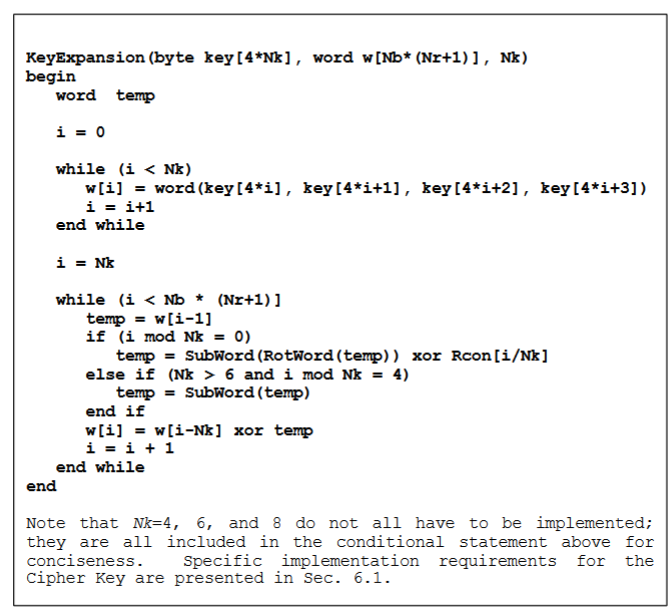
\includegraphics{media/image8.png}

Viene allocato uno \textbf{scratchpad} di 2097152 bytes.{[}\^{}22{]}
Dall'output di Keccak vengono estratti i byte \texttt{64...191} e divisi
in 8 blocchi di 16 byte ciascuno. Ogni blocco viene cifrato utilizzando
il seguente codice:

{[} \text{for } i \in \{0,\ldots,9\} \Rightarrow \textbackslash{}
\quad block = AES\_\{\text{round}\}(block, \mathbf{K}\_i) {]}

\subsubsection{Funzione cifratura AES}\label{funzione-cifratura-aes}

La funzione \texttt{aes\_round} esegue un round di cifratura AES, che
consiste nell'eseguire i passaggi seguenti sul blocco:

\begin{itemize}
\tightlist
\item
  SubBytes: ogni byte del blocco viene sostituito con un valore criptato
  utilizzando una tabella di sostituzione \emph{S-Box}.
\item
  ShiftRows: le righe del blocco vengono spostate di una posizione.
\item
  MixColumns: le colonne del blocco vengono mescolate utilizzando una
  matrice 4x4 nota come MDS{[}23\^{}{]}, progettata per essere difficile
  da invertire.
\item
  Infine, il risultato è XORato con la chiave specifica per quel round.
  A differenza della classica funzione AES per cifrare, il primo e
  l'ultimo round quando si usano le \emph{round-keys} non sono speciali.
\end{itemize}

I blocchi che ne risultano vengono riportati nei primi 128 byte dello
scratchpad. Questi ultimi vengono cifrati nuovamente nello stesso modo,
e il risultato viene scritto nei successivi 128 byte. Questa operazione
viene effettuata 10 volte, per riempire tutto lo scratchpad di dati
pseudo-randomici. I byte \texttt{64..191}, che chiameremo
\emph{payload}, sono cifrati in questo modo 10 volte. Questo diagramma
mostra le operazioni effettuate in questa prima parte

\begin{verbatim}
                               +-----+
                               |Input|
                               +-----+
                                  |
                                  V
                             +--------+
                             | Keccak |
                             +--------+
                                  |
                                  V
   +-------------------------------------------------------------+
   |                         Final state                         |
   +-------------+--------------+---------------+----------------+
   | Bytes 0..31 | Bytes 32..63 | Bytes 64..191 | Bytes 192..199 |
   +-------------+--------------+---------------+----------------+
          |                             |
          V                             |
   +-------------+                      V
   | Round key 0 |------------+---+->+-----+
   +-------------+            |   |  |     |
   |      .      |            |   |  |     |
   |      .      |            |   |  | AES |
   |      .      |            |   |  |     |
   +-------------+            |   |  |     |
   | Round key 9 |----------+-|-+-|->+-----+                 +---+
   +-------------+          | | | |     |                    |   |
                            | | | |     +------------------->|   |
                            | | | |     |                    |   |
                            | | | |     V                    |   |
                            | | | +->+-----+                 |   |
                            | | |    |     |                 | S |
                            | | |    |     |                 |   |
                            | | |    | AES |                 | c |
                            | | |    |     |                 |   |
                            | | |    |     |                 | r |
                            | | +--->+-----+                 |   |
                            | |         |                    | a |
                            | |         +------------------->|   |
                            | |         .                    | t |
                            | |         .                    |   |
                            | |         .                    | c |
                            | |         +------------------->|   |
                            | |         |                    | h |
                            | |         V                    |   |
                            | +----->+-----+                 | p |
                            |        |     |                 |   |
                            |        |     |                 | a |
                            |        | AES |                 |   |
                            |        |     |                 | d |
                            |        |     |                 |   |
                            +------->+-----+                 |   |
                                        |                    |   |
                                        +------------------->|   |
                                                             |   |
                                                             +---+
\end{verbatim}

Successivamente farò un immagine su questa cosa, ricordatemelo.

\subsection{Seconda parte: Loop
memory-hard}\label{seconda-parte-loop-memory-hard}

La seconda parte si compone di un algoritmo che mantiene lo stato
composto da 52488 iterazioni{[}\^{}24{]}. Si utilizzano operazioni
CPU-friendly, come la cifratura AES, XOR, moltiplicazioni e addizioni di
8 byte, per avere come unico

Prima di eseguire il loop utilizzato per rendere questa funzione di hash
\emph{memory-hard}, viene eseguito lo XOR sui byte \texttt{0..31} e i
byte \texttt{32..63} dell'output dell'hashing Keccak. I 32 byte
risultanti vengono utilizzati per inizializzare due variabili da 16 byte
ciascuna, \texttt{a} e \texttt{b}. Queste variabili vengono utilizzate
nel loop principale, composte da quattro passaggi:

\begin{enumerate}
\def\labelenumi{\arabic{enumi}.}
\item
  Il codice calcola l'indirizzo di memoria della variabile \texttt{a} e
  lo scrive sullo scratchpad. Per convertire un valore di 16 byte in un
  indirizzo nello scratchpad, bisogna interpretarlo come un intero
  rappresentato in little-endian, con gli ultimi 21 bit che
  rappresentano l'indice all'interno dei byte; gli ultimi 4 bit vengono
  comunque cancellati per ottenere l'allinamento a 16 byte, dato che i
  dati vengono letti e scritti sullo scratchpad in blocchi da 16 byte.
\item
  Successivamente, viene applicatata la funzione per cifrare il blocco
  \texttt{aes\_round} sull'indirizzo letto dallo scratchpad, con il
  valore di \texttt{a} usato come chiave.
\item
  Il risultato di questa operazione passa da uno XOR e il valore della
  variabile \texttt{b}, oltre ad essere scritto sullo scratchpad, sempre
  come indirizzo di memoria.
\item
  L'indirizzo ricavato viene letto dallo scratchpad e viene effettuata
  l'operazione di moltiplicazione chiamata \texttt{8byte\_mul}. Questa
  funzione, usa i primi 8 byte di ogni argomento, interpretati da essa
  come \texttt{uint\_64}, con rappresentazione little-endian. Il
  risultato di questa operazione viene convertito in 16 byte,
  concludendo l'operazione di moltiplicazione scambiando le due metà del
  risultato (8 byte ciascuna)
\item
  Il valore di \texttt{a} viene aggiunto, componente per componente in
  modulo 2\^{}64, al risultato della moltiplicazione con le due metà già
  scambiate attraverso la funzione \texttt{8byte\_add} che utilizza i
  primi 64 bit come intero senza segno, con il risultato che viene
  portato in 16 byte e scritto nello scratchpad.
\item
  Infine, viene letto l'indirizzo del risultato della cifratura
  dell'indirizzo della variabile di \texttt{a}, utilizzando come chiave
  \texttt{a} (il risultato del secondo passaggio) e viene effettuata un
  operazione di XOR con il risultato della addizione precedente.
\item
  Il risultato dell'operazione 6 viene utilizzato come nuovo valore
  della variabile \texttt{a}, mentre il risultato del passaggio 2 viene
  utilizzato come nuova variabile \texttt{b}.
\end{enumerate}

Il diagramma presente illustra le operazioni eseguite nel loop
\emph{memory-hard}:

\begin{verbatim}
   +-------------------------------------------------------------+
   |                         Final state                         |
   +-------------+--------------+---------------+----------------+
   | Bytes 0..31 | Bytes 32..63 | Bytes 64..191 | Bytes 192..199 |
   +-------------+--------------+---------------+----------------+
          |             |
          |   +-----+   |
          +-->| XOR |<--+
              +-----+
               |   |
          +----+   +----+
          |             |
          V             V
        +---+         +---+
        | a |         | b |
        +---+         +---+
          |             |
   --------------------- REPEAT 524288 TIMES ---------------------
          |             |                            address +---+
          +-------------|----------------------------------->|   |
          |   +-----+   |                               read |   |
          +-->| AES |<--|------------------------------------|   |
          |   +-----+   V                                    |   |
          |      |   +-----+                                 | S |
          |      +-->| XOR |                                 |   |
          |      |   +-----+                           write | c |
          |      |      |    +------------------------------>|   |
          |      |      +----+                       address | r |
          |      +------------------------------------------>|   |
          |      |  +-----------+                       read | a |
          |      +->| 8byte_mul |<--+------------------------|   |
          |      |  +-----------+   |                        | t |
          |      |        |         |                        |   |
          |      |        V         |                        | c |
          |      |  +-----------+   |                        |   |
          +------|->| 8byte_add |   |                        | h |
                 |  +-----------+   |                        |   |
                 |        |         |                  write | p |
                 |        +---------|----------------------->|   |
                 |        |         |                        | a |
                 |        V         |                        |   |
                 |     +-----+      |                        | d |
                 |     | XOR |<-----+                        |   |
                 |     +-----+                               |   |
                 +------+ |                                  |   |
          +-------------|-+                                  |   |
          |             |                                    +---+
   -------------------------- END REPEAT -------------------------
\end{verbatim}

\subsection{Terza parte: Calcolo del
risultato}\label{terza-parte-calcolo-del-risultato}

Dopo aver effettuato le operazioni memory-hard, i byte \texttt{32..63}
dati dall'hashing effettuato con Keccak vengono espansi in 10
\emph{round-keys} come nella prima parte.\\
I byte \texttt{64..191} dello stesso hashing vengono presi e viene
effettuato uno XOR con i primi 128 byte dello scratchpad. Il risultato
di questa operazione viene criptato con la funzione \texttt{aes\_round}
come nella prima parte, ma con le chiavi ricavate dall'espansione dei
byte \texttt{32..63}.\\
Il risultato di questa cifratura viene passato da uno XOR con i 128
bytes successivi dello scratchpad, cifrati nuovamente con la stessa
funzione, fino ad arrivare agli ultimi 128 byte dello scratchpad. Dopo
aver cifrato gli ultimi 128 byte viene effettuato lo XOR con gli ultimi
128 byte dello scratchpad.\\
I byte \texttt{64..191} del **Keccak state* vengono sostituiti con Il
risultato dell'operazione effettuata in precedenza. Tutti i 200 byte
dello stato di Keccak vengono passati da una permutazione, chiamata
\emph{Keccak-f}, con parametro \texttt{b\ =\ 1600}, l'implementazione
più sicura. Questa operazione viene effettuate per mescolare i bit dello
stato Keccak, in modo da rendere difficile la criptoanalisi del flusso
di dati.\\
Infine, i due bit più a destra vengono utilizzati per selezionare una
funzione di hash: - 0: BLAKE-256 {[}5\^{}{]} - 1: Groest1-256
{[}6\^{}{]} - 2: JH-256 {[}7\^{}{]} - 3: Skein-256 {[}8\^{}{]}

L'output di questa funzione di hash viene applicato al Keccak state, e
l'hash risultante è l'output di CryptoNight. Il diagramma sottostante
rappresenta il calcolo del risultato:

\begin{verbatim}
 +-------------------------------------------------------------+
   |                         Final state                         |
   +-------------+--------------+---------------+----------------+
   | Bytes 0..31 | Bytes 32..63 | Bytes 64..191 | Bytes 192..199 |
   +-------------+--------------+---------------+----------------+
         |                |             |                |
         |       +--------+             |                |
         |       V        |             |                |
         |+-------------+ |             |                |
         || Round key 0 |-|---+---+     |                |
         |+-------------+ |   |   |     |                |
         ||      .      | |   |   |     |                |
         ||      .      | |   |   |     |                |
         ||      .      | |   |   |     |                |
         |+-------------+ |   |   |     |                |
   +---+ || Round key 9 |-|-+-|-+ |     V                |
   |   | |+-------------+ | | | | |  +-----+             |
   |   |-|----------------|-|-|-|-|->| XOR |             |
   |   | |                | | | | |  +-----+             |
   | S | |                | | | | |     |                |
   |   | |                | | | | |     V                |
   | c | |                | | | | +->+-----+             |
   |   | |                | | | |    |     |             |
   | r | |                | | | |    |     |             |
   |   | |                | | | |    | AES |             |
   | a | |                | | | |    |     |             |
   |   | |                | | | |    |     |             |
   | t | |                | | | +--->+-----+             |
   |   | |                | | |         |                |
   | c | |                | | |         V                |
   |   | |                | | |      +-----+             |
   | h |-|----------------|-|-|----->| XOR |             |
   |   | |                | | |      +-----+             |
   | p | |                | | |         |                |
   |   | |                | | |         .                |
   | a | |                | | |         .                |
   |   | |                | | |         .                |
   | d | |                | | |         |                |
   |   | |                | | |         V                |
   |   | |                | | |      +-----+             |
   |   |-|----------------|-|-|----->| XOR |             |
   |   | |                | | |      +-----+             |
   +---+ |                | | |         |                |
         |                | | |         V                |
         |                | | +----->+-----+             |
         |                | |        |     |             |
         |                | |        |     |             |
         |                | |        | AES |             |
         |                | |        |     |             |
         |                | |        |     |             |
         |                | +------->+-----+             |
         |                |             |                |
         V                V             V                V
   +-------------+--------------+---------------+----------------+
   | Bytes 0..31 | Bytes 32..63 | Bytes 64..191 | Bytes 192..199 |
   +-------------+--------------+---------------+----------------+
   |                       Modified state                        |
   +-------------------------------------------------------------+
                                  |
                                  V
                            +----------+
                            | Keccak-f |
                            +----------+
                             |    |
                 +-----------+    |
                 |                |
                 V                V
          +-------------+  +-------------+
          | Select hash |->| Chosen hash |
          +-------------+  +-------------+
                                  |
                                  V
                          +--------------+
                          | Final result |
                          +--------------+
\end{verbatim}

\section{Problemi di CryptoNight}\label{problemi-di-cryptonight}

{[}1\^{}{]} Tatsuaki Okamoto, Kazuo Ohta, ``Universal Electronic Cash,''
Advances in Cryp-tology \textbar{} CRYPTO '91, LNCS 576, pp.~324-337,
1991.

{[}2\^{}{]} Hart, P. E.; Nilsson, N. J.; Raphael, B. (1968). ``A Formal
Basis for the Heuristic Determination of Minimum Cost Paths''. IEEE
Transactions on Systems Science and Cybernetics SSC4 4 (2): 100-107.

{[}3\^{}{]} Fergal Reid, Martin Harrigan, \An Analysis of Anonymity in
the Bitcoin System'',2012.

{[}4\^{}{]} Kay Hamacher, Stefan Katzenbeisser, \Bitcoin - An
Analysis'', 2011, http://www.youtube.com/watch?v=hlWyTqL1hFA

{[}5\^{}{]} Dorit Ron, Adi Shamir, \Quantitative Analysis of the Full
Bitcoin Transaction Graph'', 2012.

{[}6\^{}{]} https://en.bitcoin.it/wiki/Category:Mixing\_Services

{[}7\^{}{]}
http://blog.ezyang.com/2012/07/secure-multiparty-bitcoin-anonymization

{[}8\^{}{]} https://en.bitcoin.it/wiki/BIP\_0034\#Specification

{[}9\^{}{]} https://en.bitcoin.it/wiki/Mining\_hardware\_comparison

{[}10\^{}{]} https://en.bitcoin.it/wiki/Contracts

{[}11\^{}{]} https://en.bitcoin.it/wiki/Script

{[}12\^{}{]} D. Chaum and E. van Heyst (1991). ``Group signatures''.
Advances in Cryptology\textbar{} EUROCRYPT '91, volume 547 of Lecture
Notes in Computer Science. pp.~257-265.

{[}13\^{}{]} Ronald L. Rivest , Adi Shamir , Yael Tauman, How to Leak a
Secret, Proceedings of the 7th International Conference on the Theory
and Application of Cryptology and Information Security: Advances in
Cryptology, p.552-565, December 09-13, 2001

{[}14\^{}{]} Fujisaki, E., Suzuki, K.: Traceable ring signature. IEICE
Trans. of Fund. E91-A(1), 83-93 (2008); Presented in PKC 2007, LNCS 4450

{[}15\^{}{]} D. J. Bernstein, N. Duif, T. Lange, P. Schwabe, B. Yang,
\High-speed high-security signatures'',Journal of Cryptographic
Engineering, September 2012, Volume 2, Issue 2, pp 77-89

{[}16\^{}{]} Cynthia Dwork, Andrew Goldberg, and Moni Naor. On
memory-bound functions for fighting spam. In Advances in Cryptology
\textbar{} CRYPTO 2003, volume 2729 of Lecture Notes in Computer
Science, pages 426-444. Springer, 2003.

{[}17\^{}{]} Fabien Coelho, Exponential Memory-Bound Functions for Proof
of Work Protocols, 2005

{[}18\^{}{]} Colin Percival, Stronger Key Derivation via Sequential
Memory-Hard Functions, presented at BSDCan'09, May 2009

{[}19\^{}{]} http://litecoin.org

{[}20\^{}{]}{[}https://nvlpubs.nist.gov/nistpubs/FIPS/NIST.FIPS.197.pdf{]}

{[}21\^{}{]}{[}https://cryptonote.org/cns/cns008.txt{]}

{[}22\^{}{]}{[}https://keccak.team/files/NoteOnKeccakParametersAndUsage.pdf{]}

{[}23\^{}{]}{[}https://docs.monero.study/proof-of-work/cryptonight/{]}

\end{document}
